\documentclass[9pt,twocolumn,twoside]{../../styles/osajnl}
\usepackage{fancyvrb}
\journal{i524} 

\title{Heroku}

\author[1,*, +]{Yatin Sharma}

\affil[1]{School of Informatics and Computing, Bloomington, IN 47408, U.S.A.}

\affil[*]{Corresponding authors: yatins@indiana.edu}

\affil[+]{HID - S17-IR-2034}

\dates{Paper-002, \today}

\ociscodes{Heroku, PaaS, Dyno, Dyno Manifold, Logplex, Toolbeit client, Procfile.}

% replace this with your url in github/gitlab
\doi{\url{https://github.com/yatinsharma7/sp17-i524/tree/master/paper2/S17-IR-2034/report.pdf}}


\begin{abstract}
	Heroku is a cloud application program that enables developers to build and
	deploy application in almost any language. It provides everything a developer
	would need  to build customer facing application.The core of Heroku is called
	Dyno, which can be thought of as virtual machine that runs just your
	application.Dynos are scalable according to our needs as well.  
	\newline
\end{abstract}

\setboolean{displaycopyright}{true}

\begin{document}

\maketitle

\section{Introduction}
	Heroku\cite{Heroku} is Platform as a Service(Paas)\cite{PaaS} that enables us to
	build application in any language on demand. It allows us to deploy web
	applications seamlessly as well as monitor and share with other developers at
	the click of a button. It is all about rapid application development for the
	cloud, using the underlying platform infrastructure and software add-ons to
	build, deploy and monitor large and scalable web application. At present it
	handles 5 billion requests per day.
	
\section{Benefits}
	Heroku is language agnostics and provides great flexibility in choosing an
	appropriate programming language to develop the web application. It has core
	support for Ruby, Java, Python, Node.js, and PHP. Also, any other language can
	be supported by using a feature called buildpacks. Heroku provides a lot of
	flexibility in managing our applications after deployment using the Heroku
	command line tool running on the client machine or on the Heroku Infrastructure.
	Heroku is  Git\cite{Git} focused and makes it easy to share code using version
	controlling. Heroku is also a part of the Salesforce family. It has a feature
	called Heroku Connect that allows to build application that share data with the
	Salesforce deployment.

\section{Architecture}
	\begin{figure}[htbp]
		\centering
		\fbox{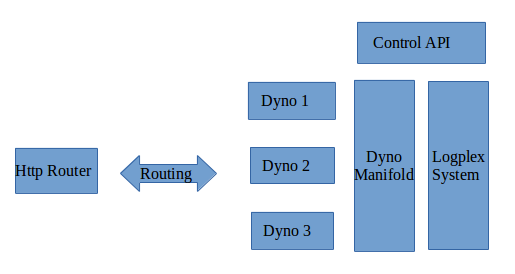
\includegraphics[width=\linewidth]{images/Heroku.png}}
		\caption{High Level Architecture of Heroku platform}
		\label{fig:Herokul-arch}
	\end{figure}
	
	The Heroku architecture consists of platform stack containing various runtime
	libraries, OS, and underlying infrastructure.The unit of work in Heroku
	framework is called Dyno. It can be thought of as packaged running version of
	our code that the application interacts with. Dynos are responsible for
	receiving web requests, writing an output and connecting to application
	resources such as databases. They are fully isolated containers running on the
	Dyno Manifold, which is the building block for execution environment. Dyno
	Manifold is responsible for process management, isolation,scaling, routing,
	distribution that are necessary for to run the web and worker processes. It is
	also fault tolerant and distributed in nature. If any dynos fails, the manifold
	restarts them automatically, hence removing a lot of maintenance hassles.

\subsection{Dyno Execution}
	 Dynos are capable of serving many request per second and execute in complete
	 isolation from each other. Each dyno gets its own virtual environment that it
	 can use to handle its own client requests. Dynos use LXC to provide container
	 like behavior to achieve complete isolation from one another.There is a memory
	 restriction of 1.5 GB per dyno, beyond which the dyno is rebooted with a
	 Heroku error which could lead to a memory leak.

\subsection{Execution Flow}
	Process type is the declaration of the command that defines the structure to be
	used while instantiating a process. Heroku has two process types- web process,
	which is responsible for handling HTTP client requests and the worker process,
	which is responsible for executing other tasks such as customer jobs of running
	background jobs and queuing tasks.



\subsection{Logging Architecture}
	Heroku logplex system provides a flexibility facility by giving us an overall
	view of our application runtime behavior. It forms the basis of the Heroku
	logging  infrastructure. It routes log streams form various sources into single
	output( for example archival system). The logplex system keeps the most recent
	data ( typically 1500 logs) that are important to extract relevant information
	from the application  being run.

\subsection{Http Routing}
	Routing Mesh are responsible for routing the web requests to the appropriate
	web process dyno. It is also responsible for seeking the application’s web dynos
	within the dyno manifold and forwarding the HTTP web requests to one of them.
	The routing mesh uses a round robin algorithm to distribute the request acroos
	various dynos. Since the dynos could be running in distributed manner, the
	routing mesh manages the access and routing internally and none of the dynos are
	statically addressable. Heroku also supports multithreaded and asynchronous
	application, accepting many network connections to process client requests.


\section{Process Architecture}
	A Heroku application can be thought of a multiple process, each consuming
	resources like a normal UNIX process, that run on the Heroku Dyno manifold.
	Heroku defines each process through configuration file called Procfile- which is
	a text file, placed in the root of the application and contains the format
	describing 	how our application will run.

\section{Heroku Platform API}
	Heroku platform API is a tool that enables us to call Heroku platform services
	and create application, plug in new add-ons simply using HTTP. It gives the
	developers complete control over their application. The three components that
	define the behavior of the API are : 1)Security 2)Schema 3)Data. The client
	accesses the API using standard methods defined for HTTP. The API then acts on
	the request and returns the result in JSON format.

\section{Security}
	Heroku employs various measures to ensure that the application and data stores
	within the platform are secure from external attacks,thefts and hacks. Heroku
	enforces SSH\cite{SSH} protocol to encrypt the source code while they are
	getting pushed into the Heroku environment. Any application that runs on Heroku
	is in complete isolation from each other, so that no two application can see
	each other getting executed. It also restricts applications from making local
	network connection between hosts. It enables data security by keeping the data
	in access controlled databases.


\section{Getting started}
	There are few prerequisites that we need to perform before we can start using
	Heroku: 1) Get Heroku account 2) Install Heroku toolbeit client\cite{Toolbeit} 
	3) Set up SSH for our user account. Heroku toolbeit is the client software
	requird to work with the Heroku platform and contains the following component:
	Heroku Client, Foreman and Git.

\section{Conclusion}
	Heroku is dramatically different from the traditional hosting or any normal
	cloud infrastructure offerings. Instead of thinking about virtual servers as
	individual units and trying to figure out how many do we need and the
	communication between them, Heroku completely abstracts the servers and
	filesystems away. As a developer we just have to push the code and heroku will 
	manage all the rest of the process. Heroku provides a complete developer
	experience and application runtime and also frees the developer from hassles of
	underlying infrastructure. It manages all that in scalable and highly
	maintainable fashion.

\section*{Acknowledgements}

	The author thanks Prof. Gregor von Laszewski for his technical guidance.

% Bibliography

\bibliography{references}

\end{document}
